\documentclass[aspectratio=169,11pt]{beamer}
\usepackage{fontspec}
\usepackage{polyglossia}
\setmainlanguage{russian}
\setsansfont[Path=fonts/,BoldFont=Onest-800.ttf]{Onest-400.ttf}
\setmainfont[Path=fonts/,BoldFont=Onest-800.ttf]{Onest-400.ttf}
\newfontfamily\cyrillicfont[Path=fonts/,BoldFont=Onest-800.ttf]{Onest-400.ttf}
\newfontfamily\cyrillicfontsf[Path=fonts/,BoldFont=Onest-800.ttf]{Onest-400.ttf}
\usepackage{graphicx}
\usepackage{tikz}
\usepackage{xfp}
\definecolor{Paper}{HTML}{FBFAF6}
\definecolor{Ink}{HTML}{202522}
\definecolor{Coral}{HTML}{D9432D}
\definecolor{Salmon}{HTML}{FFE6DF}
\definecolor{Mint}{HTML}{E9F1E9}
\definecolor{Blue}{HTML}{E9F0F8}
\definecolor{Muted}{HTML}{59635D}
\definecolor{Line}{HTML}{DBE2DA}
\setbeamercolor{normal text}{fg=Ink,bg=Paper}
\setbeamercolor{background canvas}{bg=Paper}
\setbeamertemplate{navigation symbols}{}
\setbeamertemplate{footline}{}
\hyphenpenalty=10000
\exhyphenpenalty=10000
\tolerance=10000

% Координаты 160 × 90 мм. Короткие карточки повторяют логику шаблона защиты.
\newcommand{\slidebegin}[3]{%
  \begin{tikzpicture}[remember picture,overlay,x=1mm,y=1mm]
  \begin{scope}[shift={(current page.south west)}]
  \fill[Paper] (0,0) rectangle (160,90);
  \node[anchor=west,text=Coral,font=\bfseries\fontsize{12}{14}\selectfont] at (10,84) {#1};
  \node[anchor=north west,text width=140mm,align=left,text=Ink,font=\bfseries\fontsize{18}{21}\selectfont] at (10,78) {#2};
  \draw[Line,line width=.35mm] (10,10) -- (150,10);
  \node[anchor=east,text=Muted,font=\fontsize{10}{12}\selectfont] at (150,5.6) {#3 / 18};
}
\newcommand{\slideend}{%
  \end{scope}
  \end{tikzpicture}
}
\newcommand{\panel}[5]{\fill[#5,rounded corners=2.5mm] (#1,#2) rectangle ({#1+#3},{#2+#4});}
\newcommand{\labeltext}[4]{\node[anchor=north west,text width=#3mm,align=left,text=Ink,font=\bfseries\fontsize{12}{15}\selectfont] at (#1,#2) {#4};}
\newcommand{\bodytext}[4]{\node[anchor=north west,text width=#3mm,align=left,text=Ink,font=\fontsize{10}{12.5}\selectfont] at (#1,#2) {#4};}
\newcommand{\mutedtext}[4]{\node[anchor=north west,text width=#3mm,align=left,text=Muted,font=\fontsize{10.5}{13}\selectfont] at (#1,#2) {#4};}
\newcommand{\bigfigure}[4]{\node[anchor=north west,text width=#3mm,align=left,text=Coral,font=\bfseries\fontsize{22}{25}\selectfont] at (#1,#2) {#4};}
\begin{document}

\begin{frame}[plain]
\begin{tikzpicture}[remember picture,overlay,x=1mm,y=1mm]
\begin{scope}[shift={(current page.south west)}]
\fill[Paper] (0,0) rectangle (160,90);
\node[anchor=west,text=Coral,font=\bfseries\fontsize{12}{14}\selectfont] at (10,84) {Ладно · Ярославль};
\node[anchor=north west,text width=75mm,align=left,text=Ink,font=\bfseries\fontsize{24}{28}\selectfont] at (10,65) {Ремонт дома\\без поиска мастера};
\node[anchor=north west,text width=70mm,align=left,text=Ink,font=\fontsize{12}{16}\selectfont] at (10,38) {Одна заявка. Смета до выезда. Мы сами организуем мастера и проверим работу.};
\node[anchor=west,text=Muted,font=\fontsize{10}{12}\selectfont] at (10,13) {План пилота · демо-день 2026};
\node[anchor=center,inner sep=0] at (119,44) {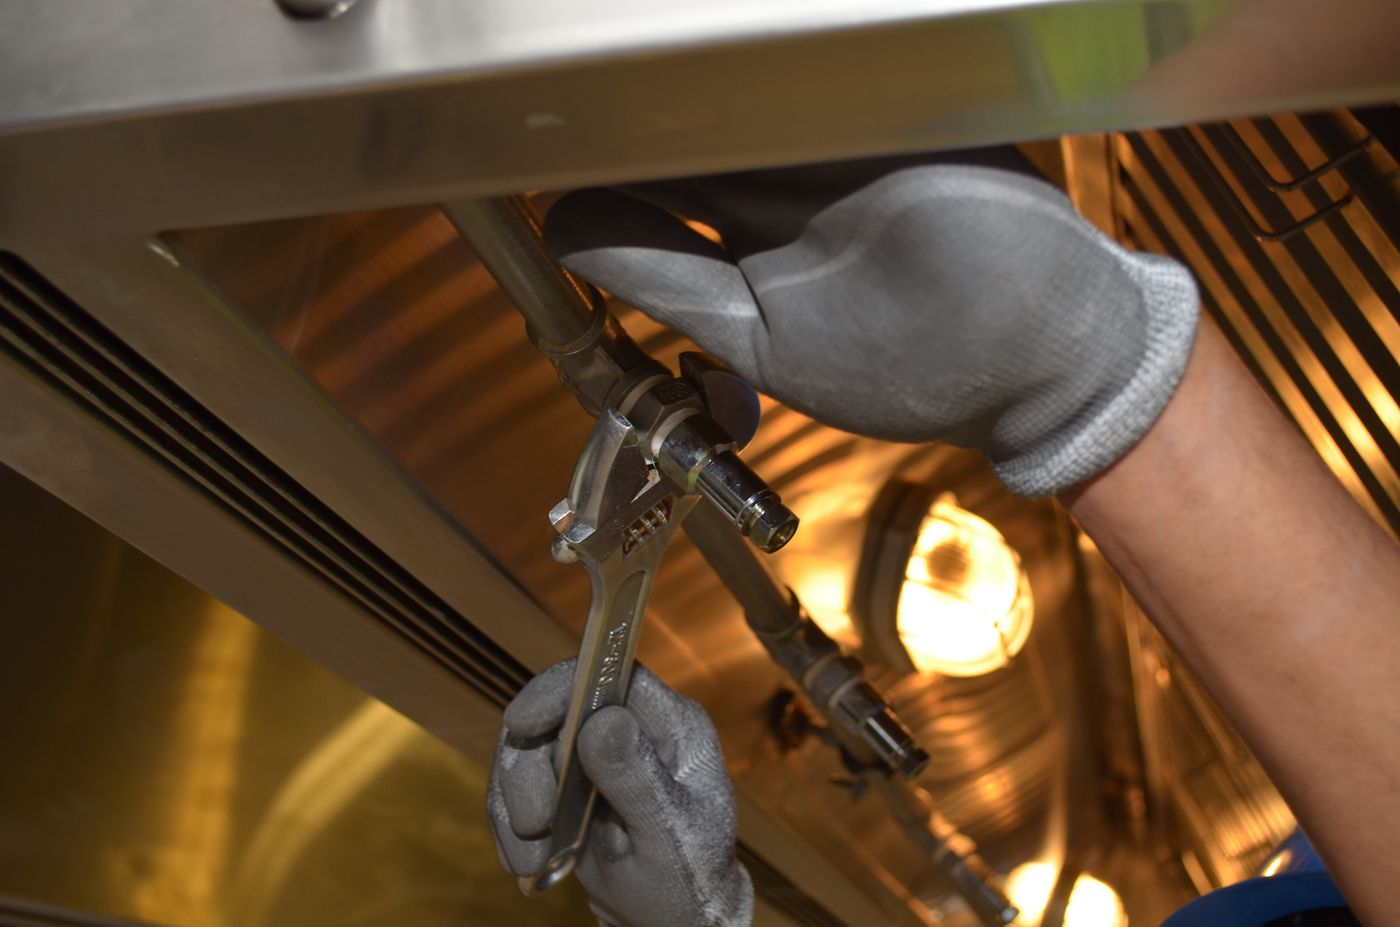
\includegraphics[width=62mm,height=59mm,keepaspectratio]{../assets/stock/pipe-repair.jpg}};
\end{scope}\end{tikzpicture}\end{frame}

\begin{frame}[plain]
\slidebegin{Проблема}{В воскресенье течёт сифон. Мастера ещё нет}{2}
\begin{scope}
\clip (88,16) rectangle (150,64);
\node[anchor=center,inner sep=0] at (119,40) {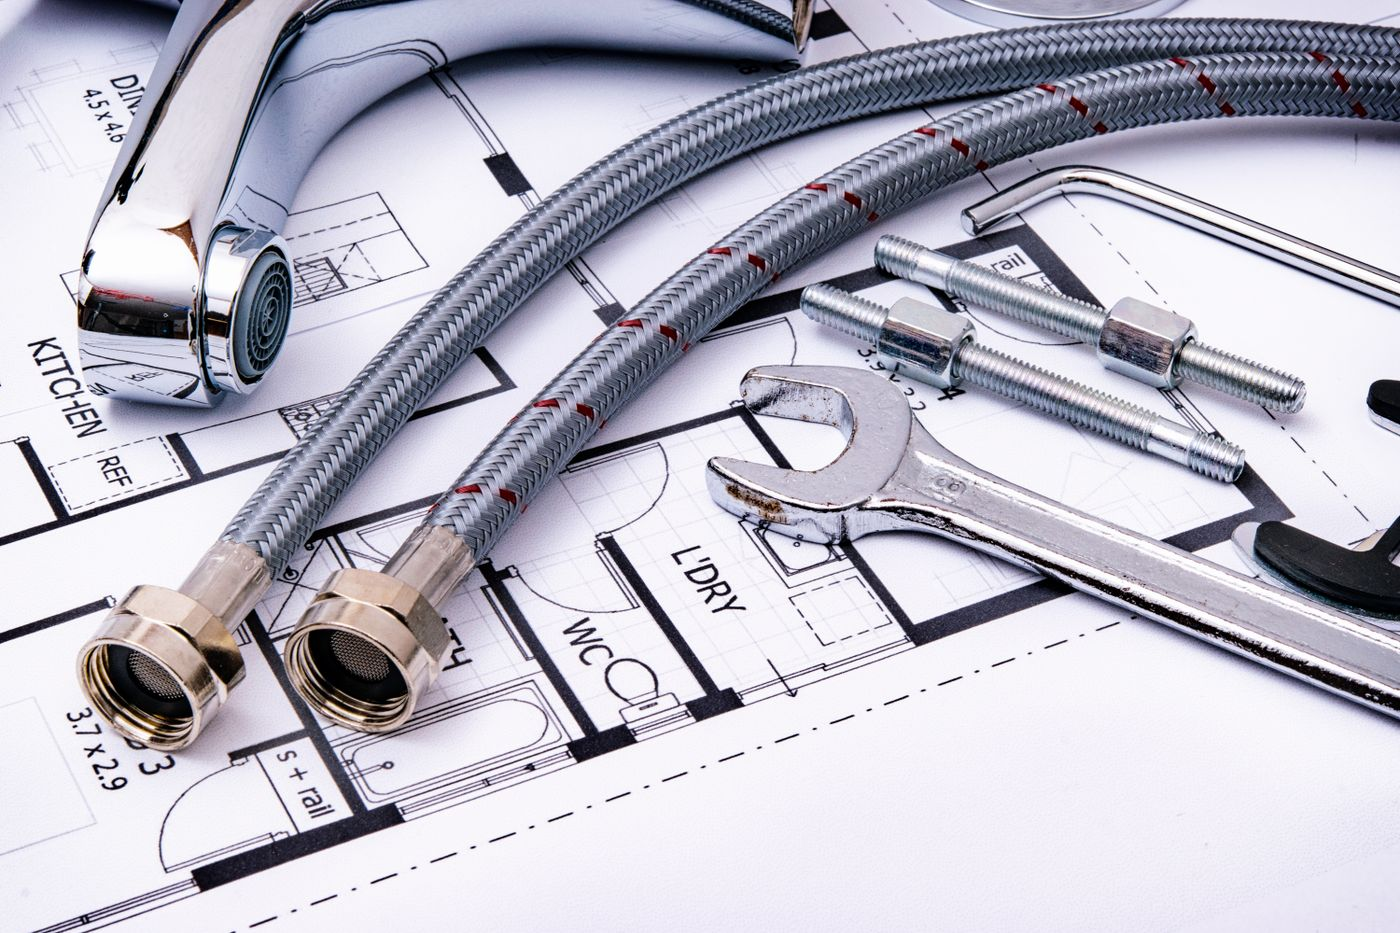
\includegraphics[height=48mm]{../assets/stock/tap.jpg}};
\end{scope}
\labeltext{10}{59}{70}{Что делает клиент}
\bodytext{10}{51}{70}{Открывает площадку, сравнивает профили и пишет нескольким людям.}
\labeltext{10}{33}{70}{Что остаётся неизвестным}
\bodytext{10}{25}{70}{Кто сможет приехать сегодня, сколько будет стоить ремонт и кто отвечает за результат.}
\slideend
\end{frame}

\begin{frame}[plain]
\slidebegin{Сейчас}{Клиент сам ведёт весь процесс}{3}
\begin{scope}
\clip (88,16) rectangle (150,64);
\node[anchor=center,inner sep=0] at (119,40) {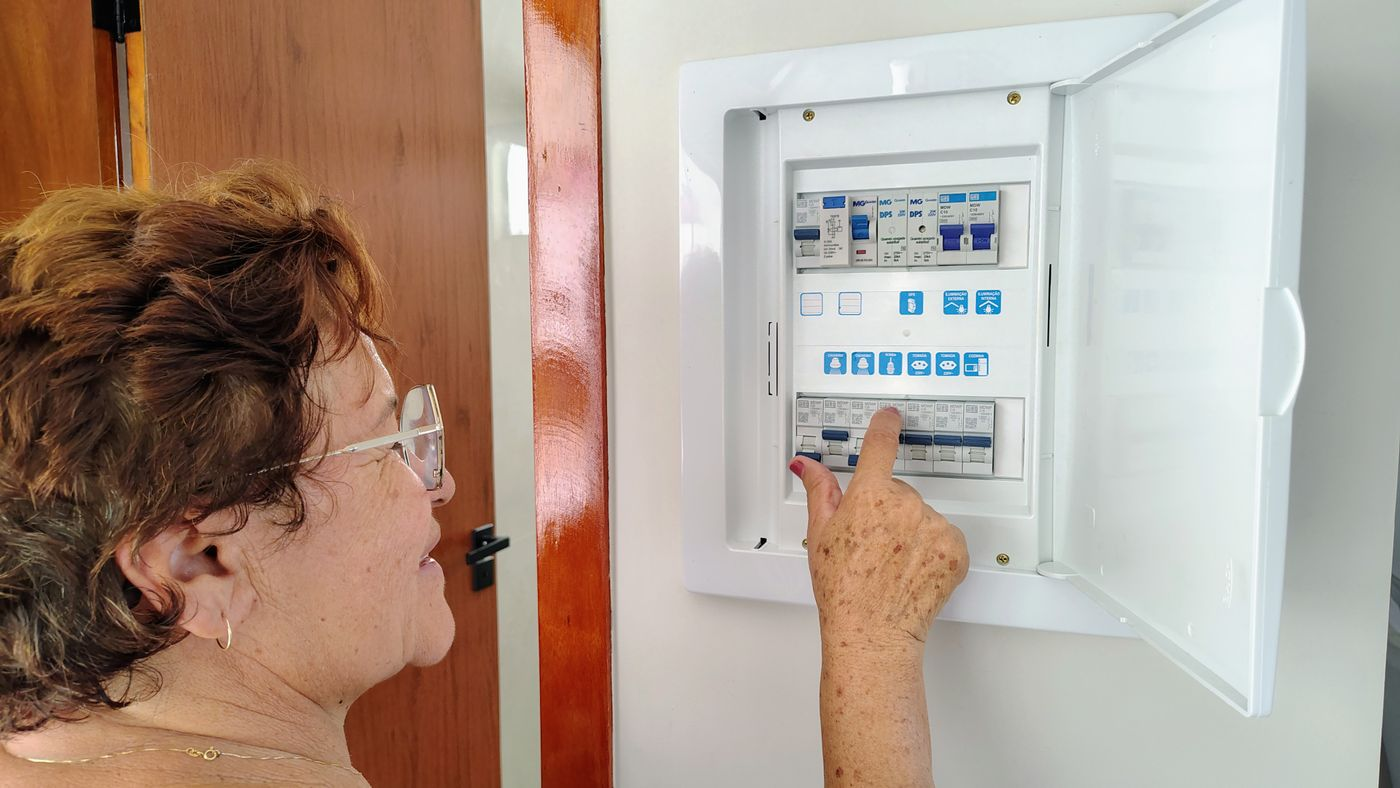
\includegraphics[height=48mm]{../assets/stock/fuse-box.jpg}};
\end{scope}
\labeltext{10}{59}{70}{Поиск и согласование}
\bodytext{10}{51}{70}{Выбирает площадку, пишет мастерам, ждёт цену и время приезда.}
\labeltext{10}{33}{70}{Приёмка}
\bodytext{10}{25}{70}{Сам проверяет работу и решает спорные вопросы.}
\slideend
\end{frame}

\begin{frame}[plain]
\slidebegin{Решение}{Клиенту достаточно одной заявки}{4}
\node[anchor=center,inner sep=0] at (119,40) {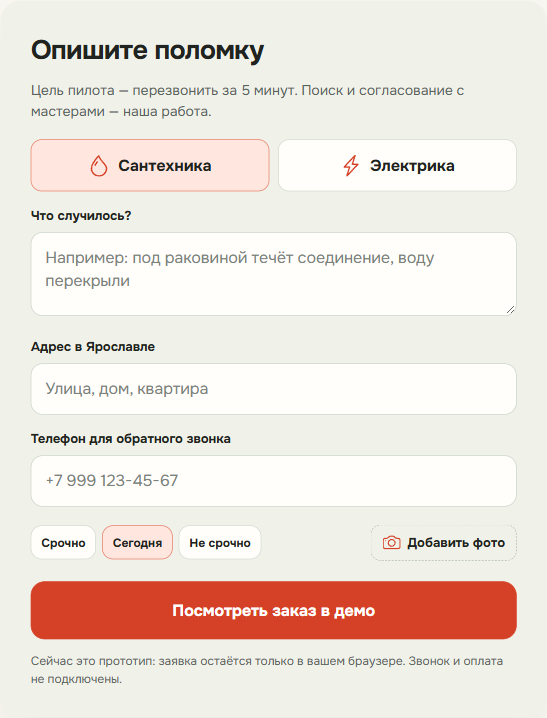
\includegraphics[width=61mm,height=48mm,keepaspectratio]{site-home-crop.png}};
\labeltext{10}{59}{70}{Клиент}
\bodytext{10}{51}{70}{Описывает поломку, прикладывает фото и оставляет телефон.}
\labeltext{10}{33}{70}{Ладно}
\bodytext{10}{25}{70}{Готовит смету, назначает мастера и ведёт заказ до результата.}
\slideend
\end{frame}

\begin{frame}[plain]
\slidebegin{После заявки}{Не ждать ответа неделями — стандарт пилота}{5}
\begin{scope}
\clip (88,16) rectangle (150,64);
\node[anchor=center,inner sep=0] at (119,40) {
\includegraphics[height=48mm]{../assets/stock/worker3.jpg}};
\end{scope}
\labeltext{10}{59}{70}{Первые минуты}
\bodytext{10}{51}{70}{Оператор должен перезвонить в течение 5 минут.}
\labeltext{10}{33}{70}{До выезда}
\bodytext{10}{25}{70}{Главный мастер готовит смету. Диспетчер назначает исполнителя.}
\slideend
\end{frame}

\begin{frame}[plain]
\slidebegin{Цена}{Смета видна до приезда мастера}{6}
\node[anchor=center,inner sep=0] at (119,40) {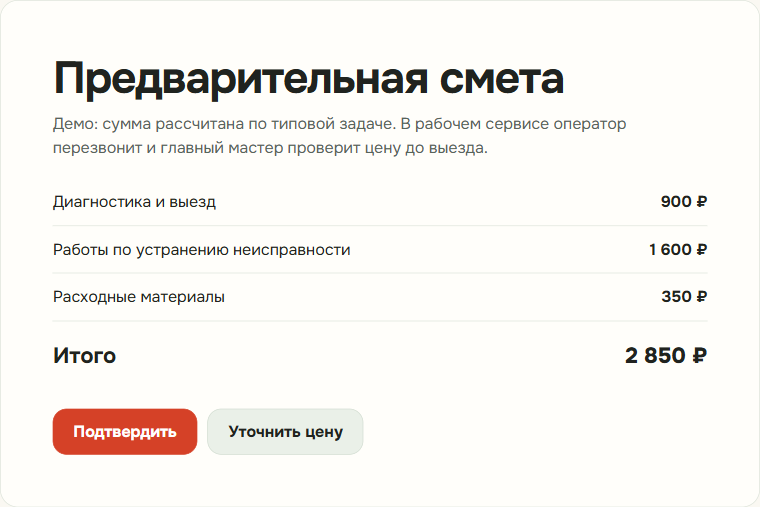
\includegraphics[width=61mm,height=48mm,keepaspectratio]{site-quote-crop.png}};
\labeltext{10}{59}{70}{В примере заказа}
\bodytext{10}{51}{70}{Выезд и диагностика — 900 ₽, работа — 1 600 ₽, материалы — 350 ₽.}
\labeltext{10}{33}{70}{Итого}
\bodytext{10}{25}{70}{2 850 ₽ до выезда. Другую работу согласуют отдельно.}
\slideend
\end{frame}

\begin{frame}[plain]
\slidebegin{Диспетчерская}{Поиск и замена мастера — наша работа}{7}
\node[anchor=center,inner sep=0] at (119,40) {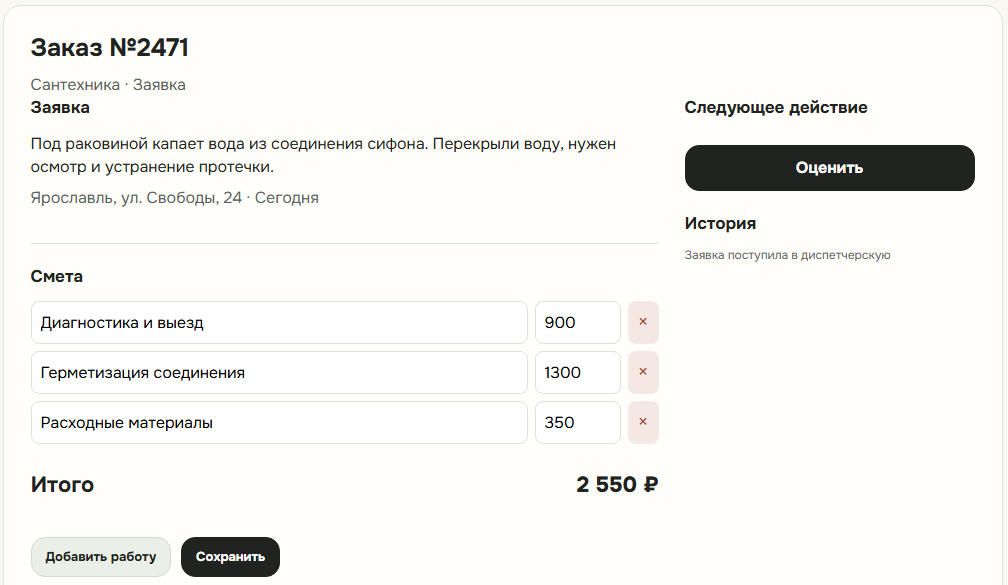
\includegraphics[width=61mm,height=48mm,keepaspectratio]{site-dispatcher-crop.png}};
\labeltext{10}{59}{70}{Назначение}
\bodytext{10}{51}{70}{Диспетчер видит фото, адрес, срочность и смету в одном заказе.}
\labeltext{10}{33}{70}{Отказ исполнителя}
\bodytext{10}{25}{70}{Система предлагает следующего подходящего мастера; клиент не начинает поиск заново.}
\slideend
\end{frame}

\begin{frame}[plain]
\slidebegin{Исполнители}{Мастера работают по одному стандарту}{8}
\begin{scope}
\clip (88,16) rectangle (150,64);
\node[anchor=center,inner sep=0] at (119,40) {
\includegraphics[width=62mm]{../assets/stock/socket-work.jpg}};
\end{scope}
\labeltext{10}{59}{70}{До допуска}
\bodytext{10}{51}{70}{Проверяем навыки и обучаем работе по чек-листу.}
\labeltext{10}{33}{70}{На заказе}
\bodytext{10}{25}{70}{Заранее знает задачу. После ремонта показывает результат и убирает мусор.}
\slideend
\end{frame}

\begin{frame}[plain]
\slidebegin{Качество}{Приёмка не заканчивается словом «готово»}{9}
\begin{scope}
\clip (88,16) rectangle (150,64);
\node[anchor=center,inner sep=0] at (119,40) {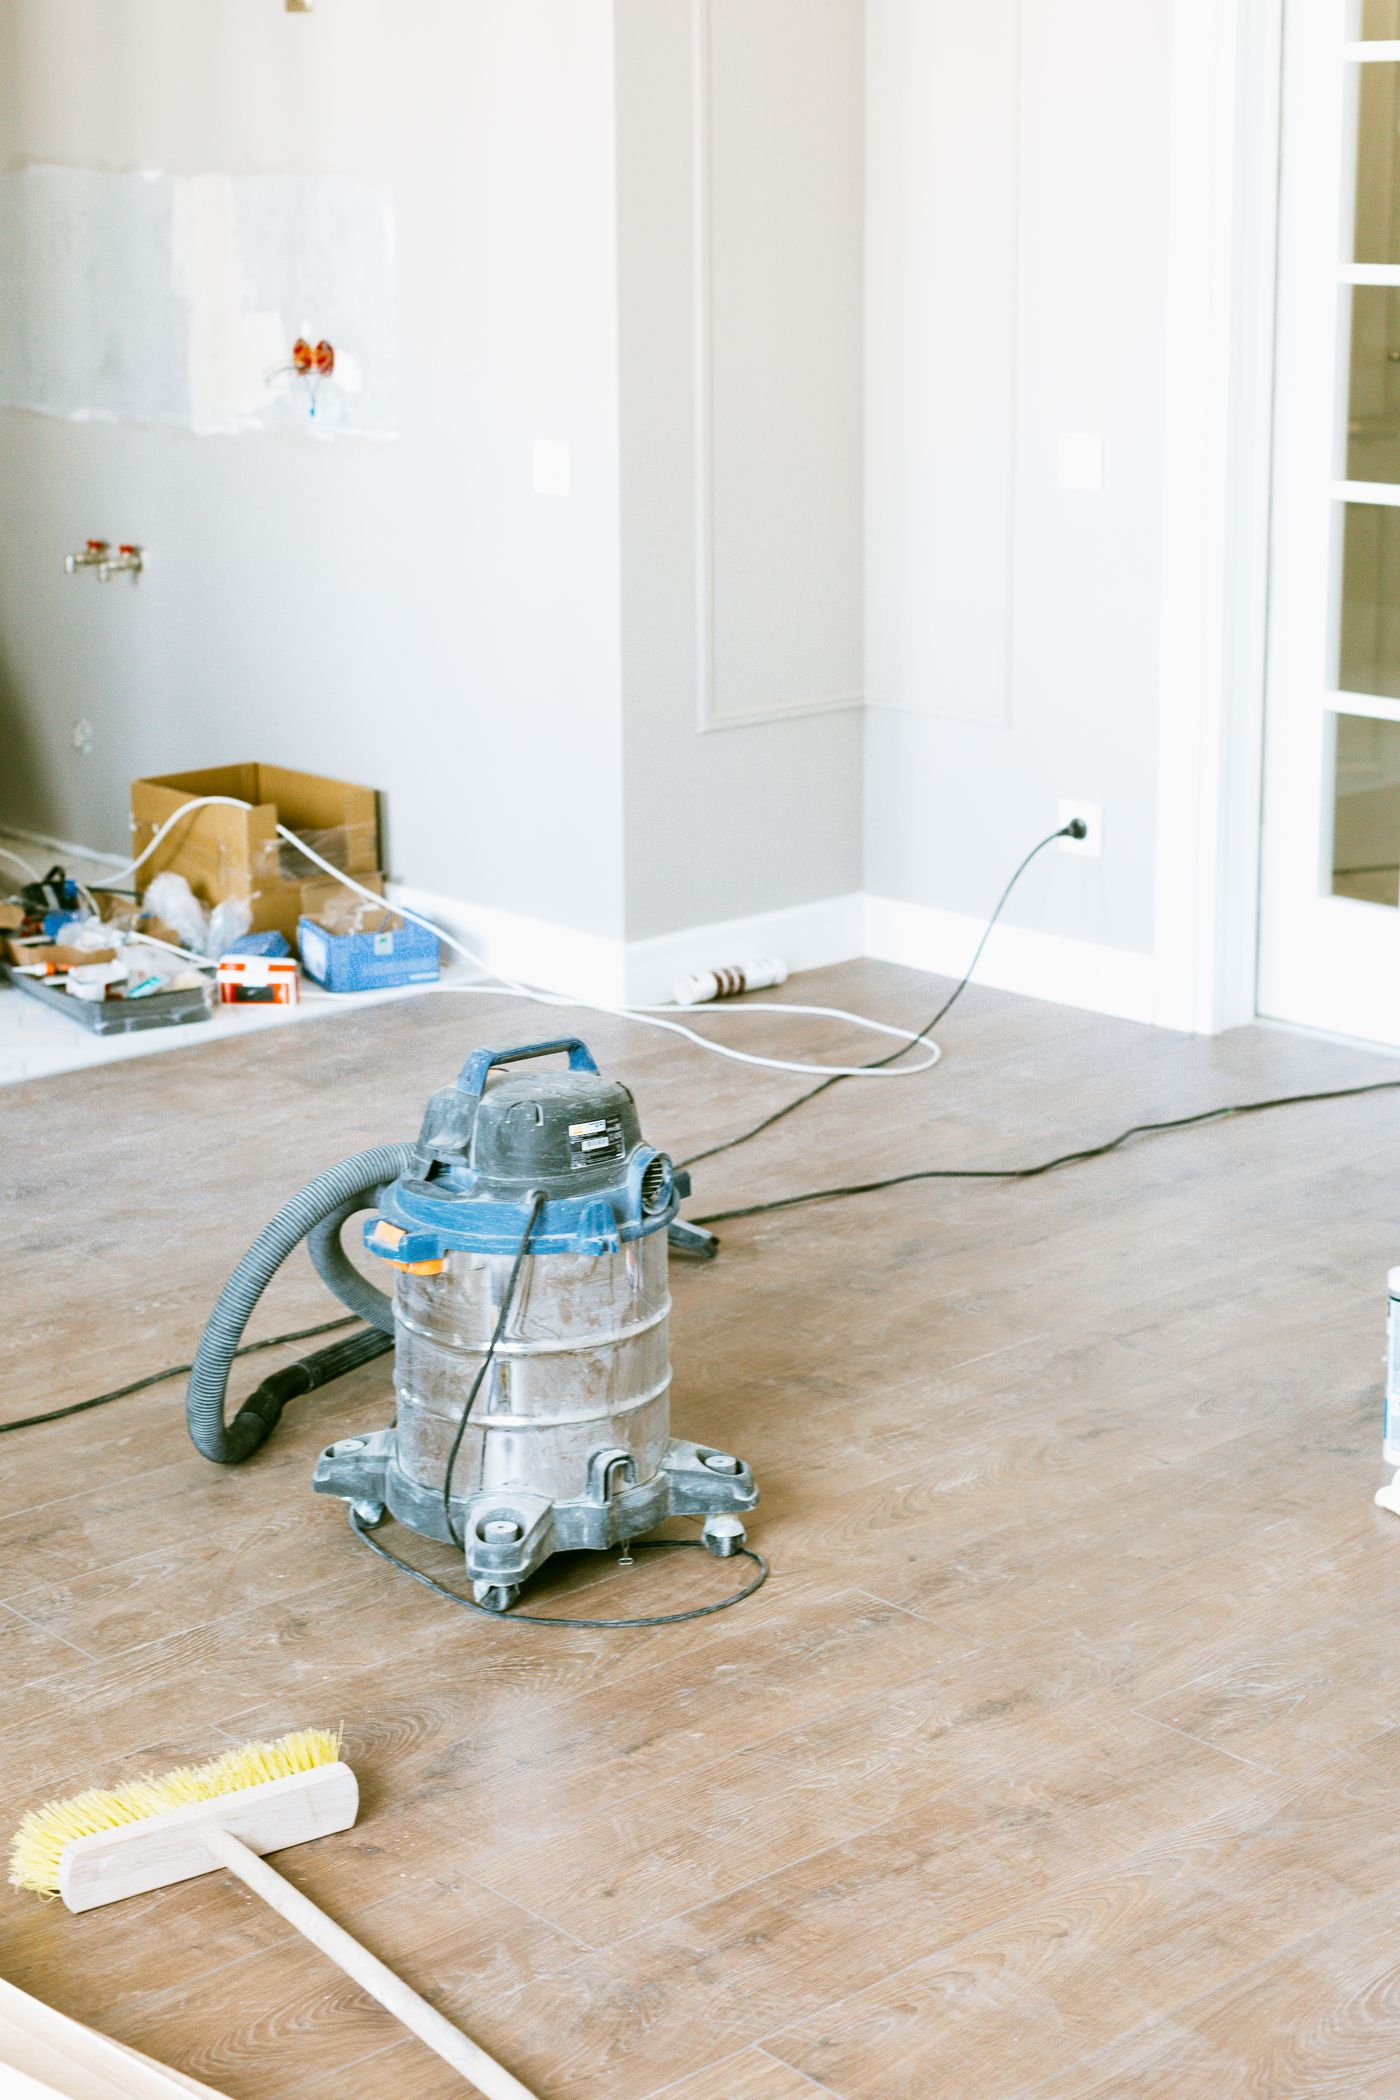
\includegraphics[width=62mm]{../assets/stock/clean-tools.jpg}};
\end{scope}
\labeltext{10}{59}{70}{Чек-лист}
\bodytext{10}{51}{70}{Проверка результата вместе с клиентом, фото до и после, уборка места работы.}
\labeltext{10}{33}{70}{Ответственность}
\bodytext{10}{25}{70}{Условия гарантии и итоговая сумма фиксируются в заказе.}
\slideend
\end{frame}

\begin{frame}[plain]
\slidebegin{Прозрачность}{Клиент видит, кто едет и что уже сделано}{10}
\begin{scope}
\clip (88,16) rectangle (150,64);
\node[anchor=center,inner sep=0] at (119,40) {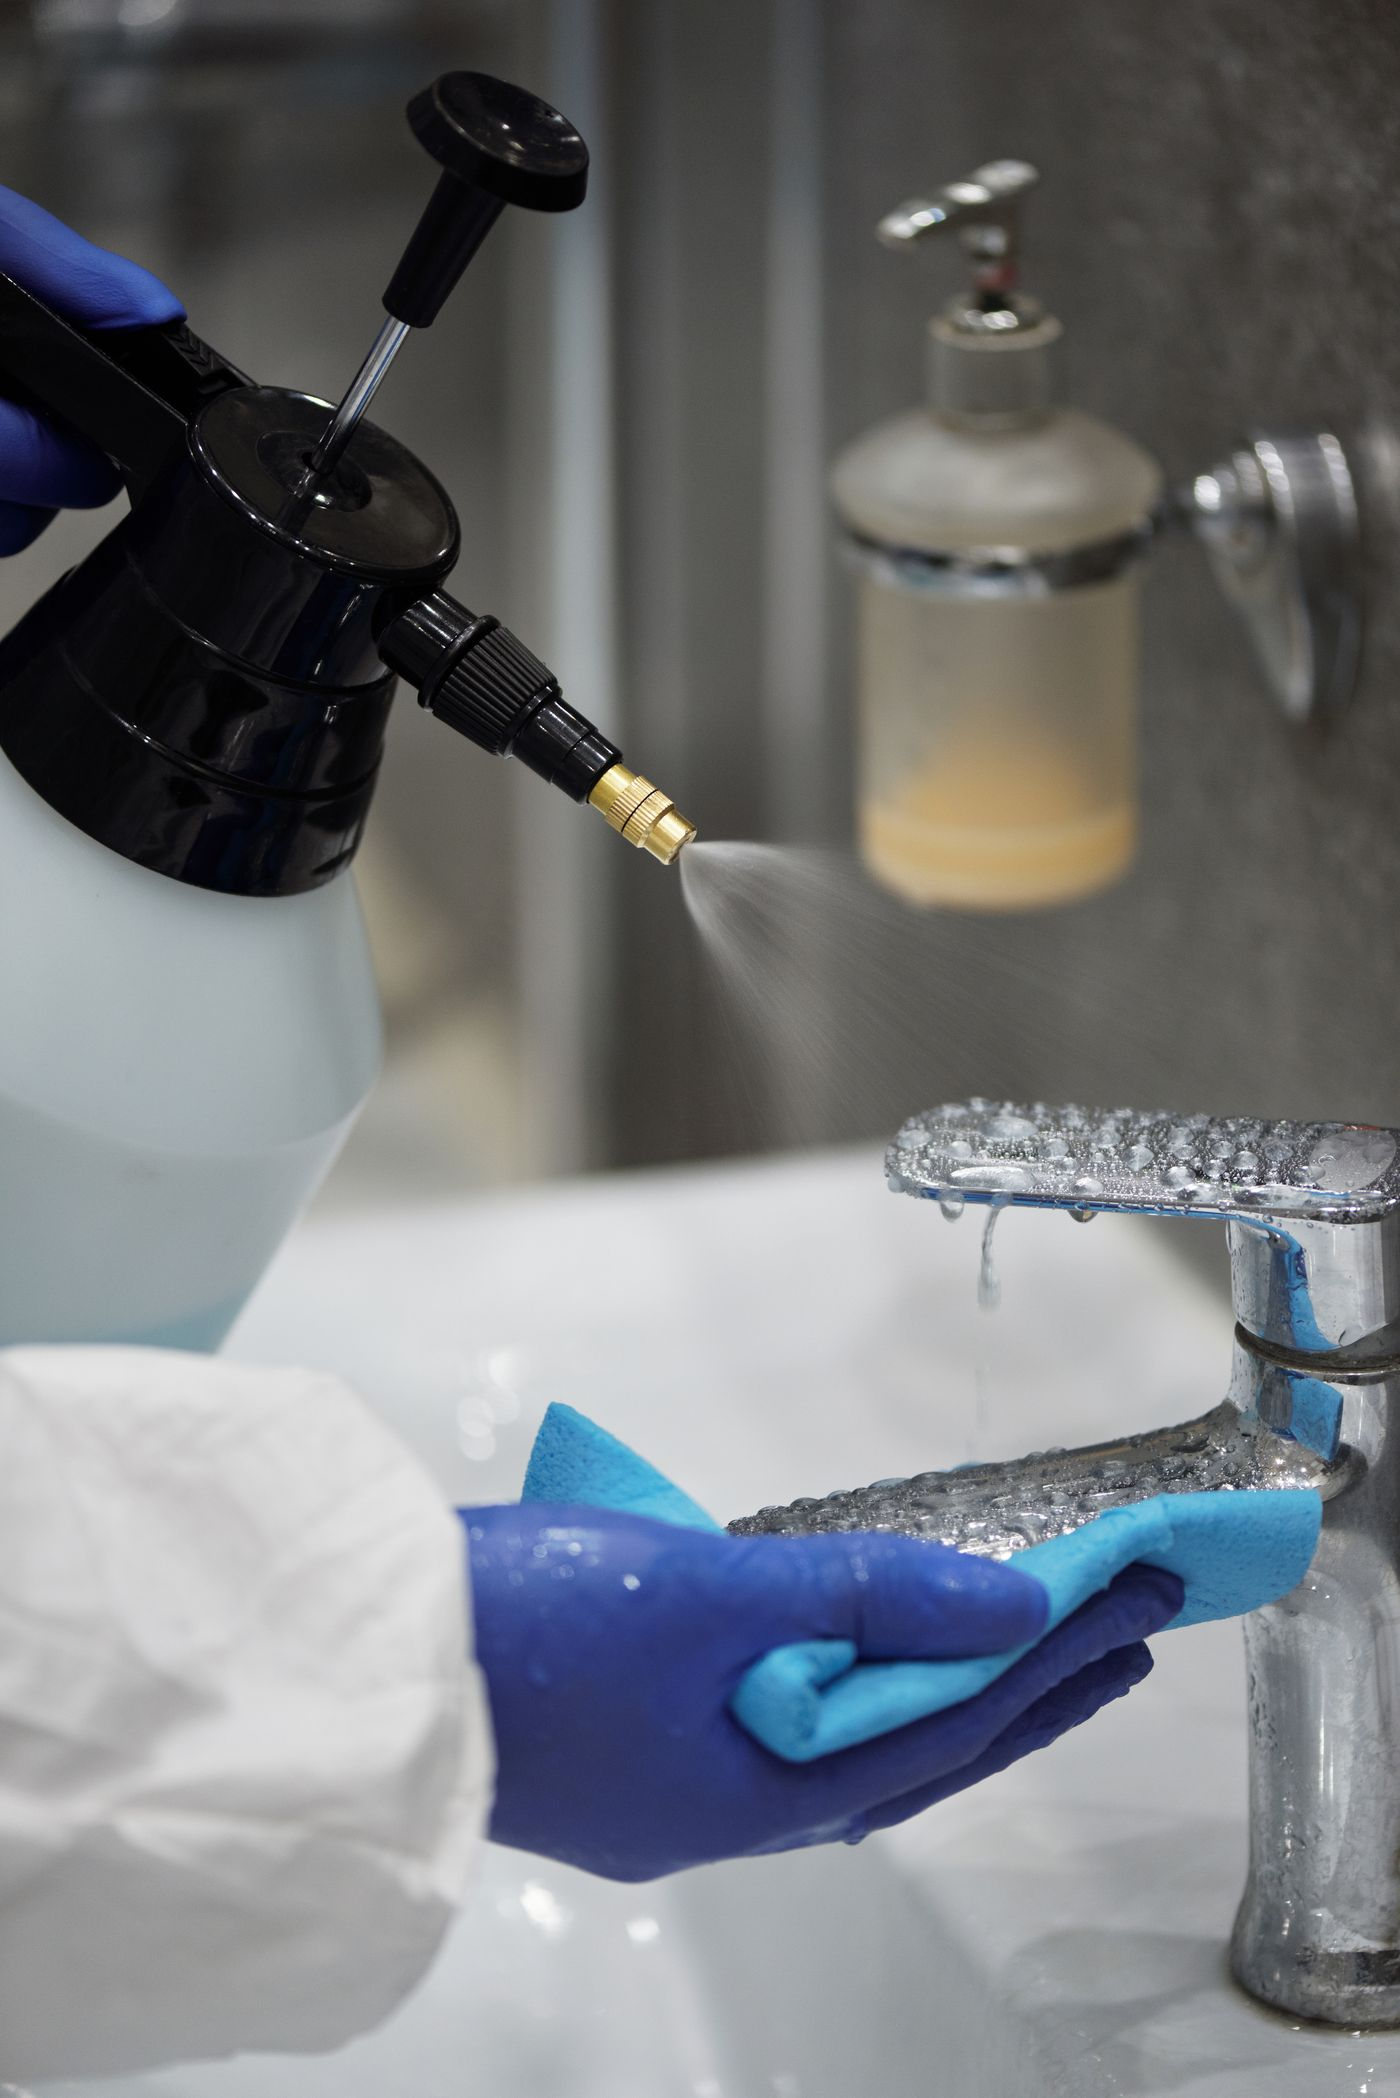
\includegraphics[width=62mm]{../assets/stock/clean-faucet.jpg}};
\end{scope}
\labeltext{10}{59}{70}{Карточка мастера}
\bodytext{10}{51}{70}{Фото, специализация, предыдущие работы и отзывы.}
\labeltext{10}{33}{70}{Заказ}
\bodytext{10}{25}{70}{Смета, этапы и фотоотчёт. Пока это показано на демо-данных.}
\slideend
\end{frame}

\begin{frame}[plain]
\slidebegin{Категории}{На старте — сантехника и электрика}{11}
\begin{scope}
\clip (88,16) rectangle (150,64);
\node[anchor=center,inner sep=0] at (119,40) {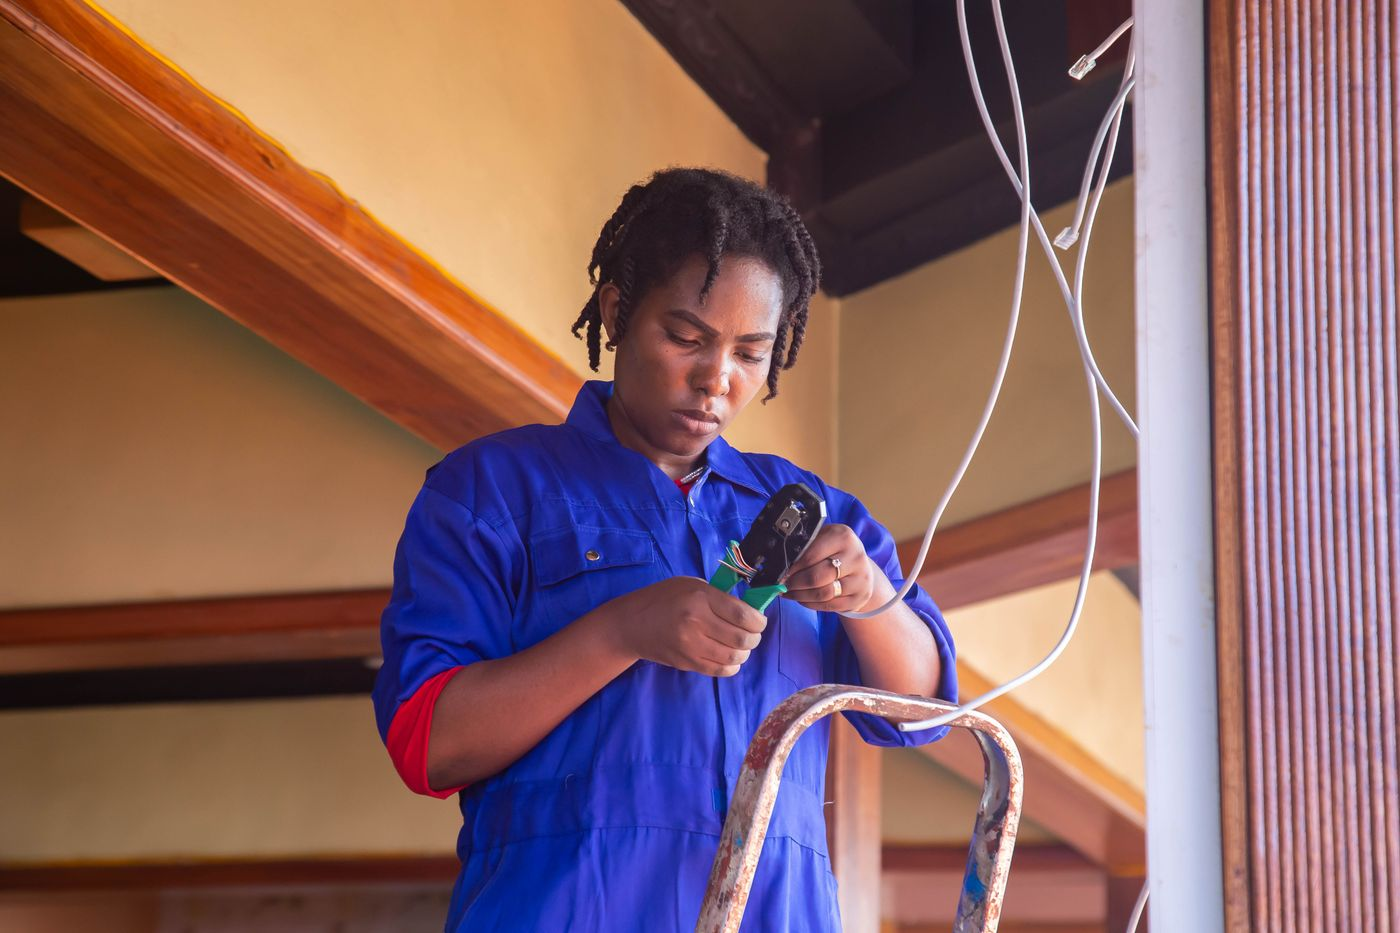
\includegraphics[height=48mm]{../assets/stock/electrician.jpg}};
\end{scope}
\labeltext{10}{59}{70}{Сантехника}
\bodytext{10}{51}{70}{Течь под раковиной, смеситель, сифон, засор.}
\labeltext{10}{33}{70}{Электрика}
\bodytext{10}{25}{70}{Розетка, свет, диагностика щита.}
\slideend
\end{frame}

\begin{frame}[plain]
\slidebegin{Скорость}{Срочные заявки — отдельный маршрут}{12}
\begin{scope}
\clip (88,16) rectangle (150,64);
\node[anchor=center,inner sep=0] at (119,40) {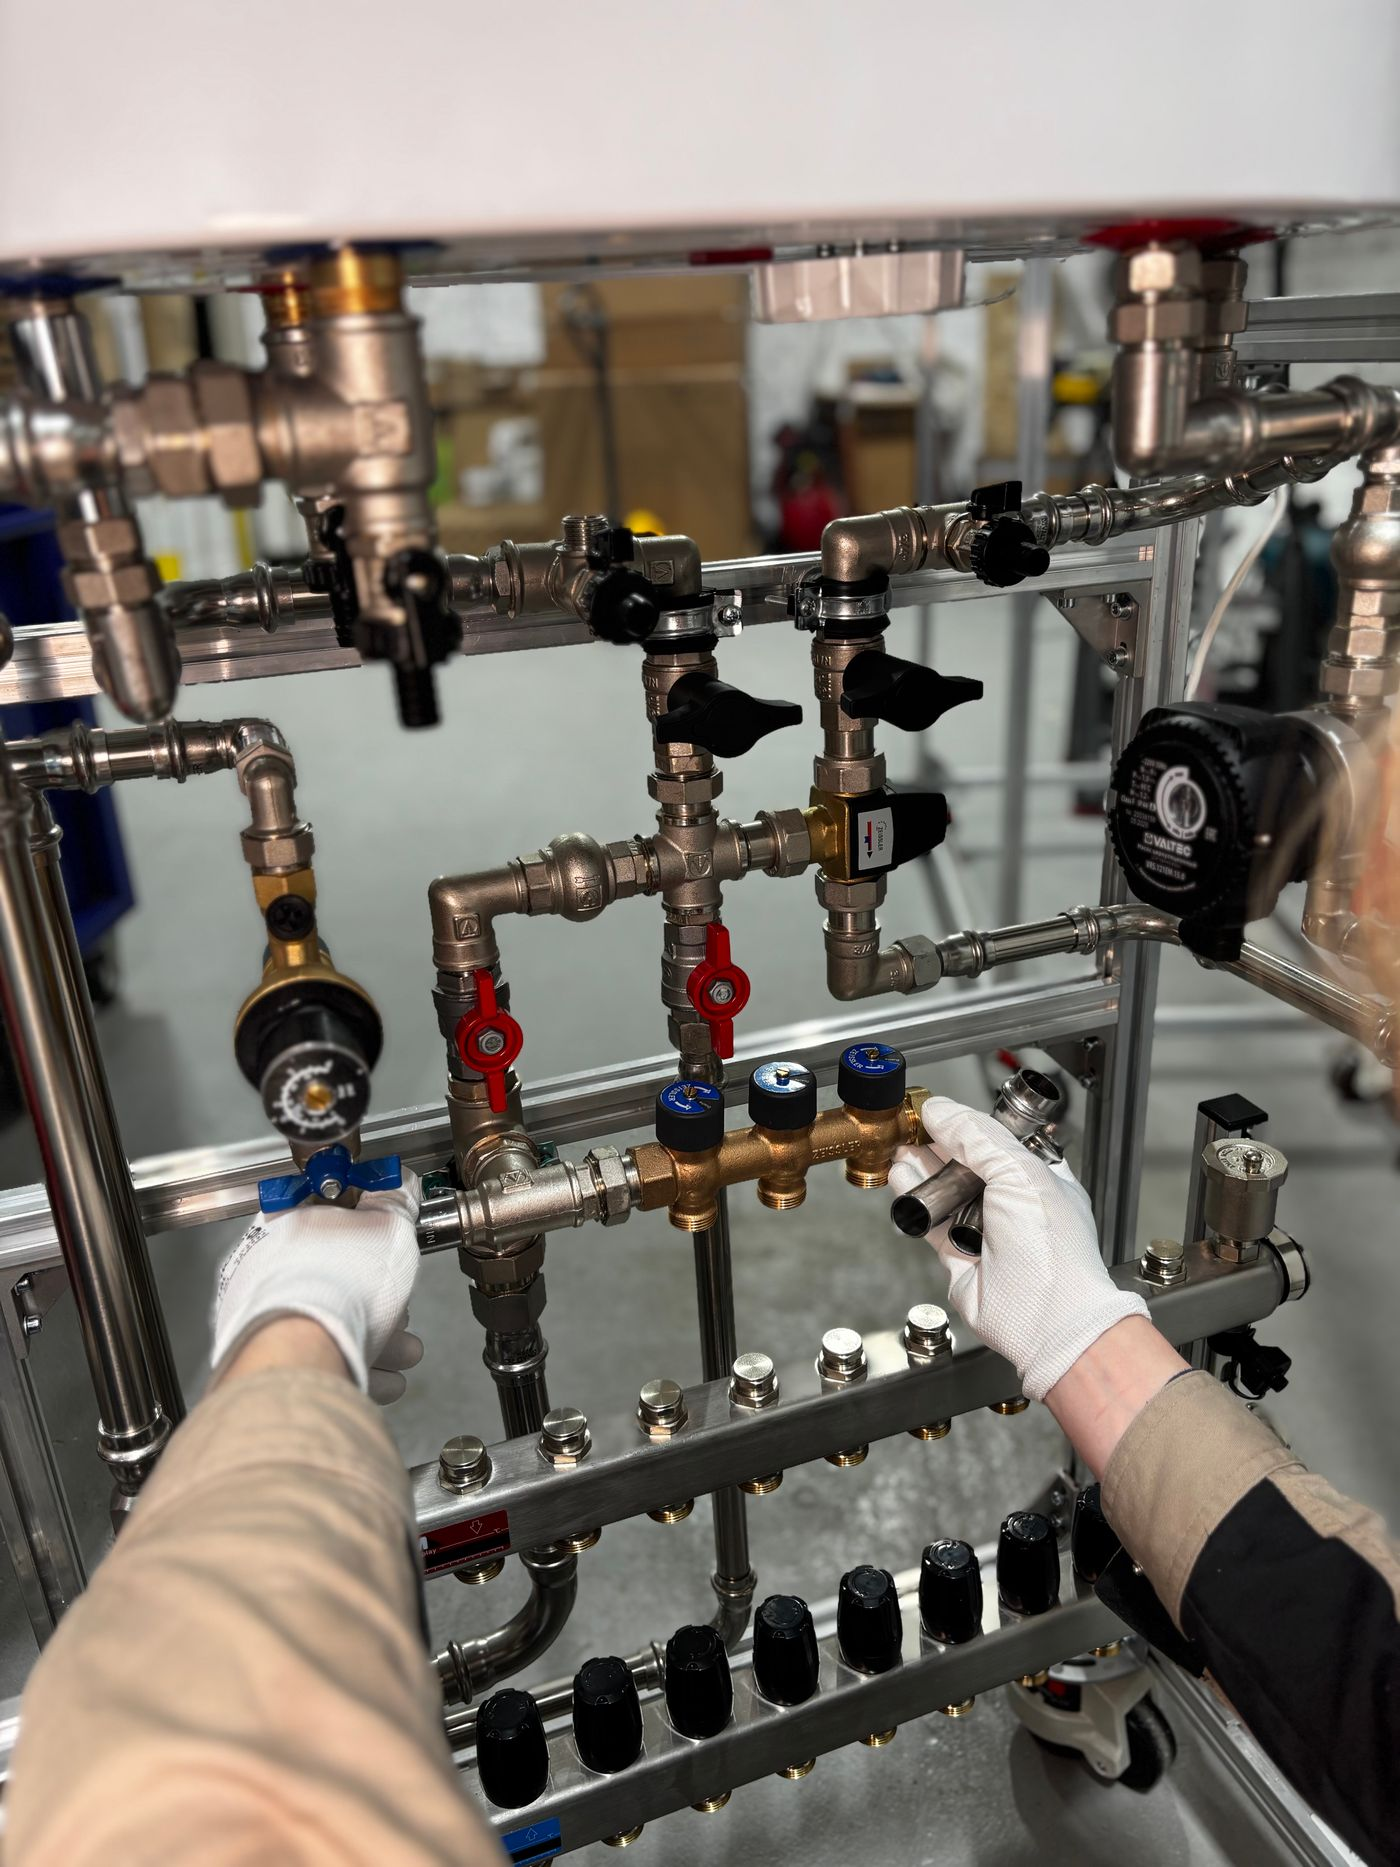
\includegraphics[width=62mm]{../assets/stock/valves.jpg}};
\end{scope}
\labeltext{10}{59}{70}{Цель}
\bodytext{10}{51}{70}{Выезд в течение часа при наличии свободного мастера.}
\labeltext{10}{33}{70}{Выходные и праздники}
\bodytext{10}{25}{70}{Нужны дежурства и резерв. Если окно занято, сразу назовём доступное время.}
\slideend
\end{frame}

\begin{frame}[plain]
\slidebegin{Ярославль}{Пилот запускаем по районам, а не «везде»}{13}
\begin{scope}
\clip (88,16) rectangle (150,64);
\node[anchor=center,inner sep=0] at (119,40) {
\includegraphics[width=62mm]{../assets/stock/yaroslavl.jpg}};
\end{scope}
\labeltext{10}{59}{70}{Первый контур}
\bodytext{10}{51}{70}{Кировский, Ленинский и Фрунзенский районы: проверяем маршруты и доступность мастеров.}
\labeltext{10}{33}{70}{Затем}
\bodytext{10}{25}{70}{Расширение на Дзержинский и Красноперекопский районы после замера времени выезда.}
\slideend
\end{frame}

\begin{frame}[plain]
\slidebegin{Первые заявки}{Конкретные каналы для старта}{14}
\labeltext{10}{61}{138}{Яндекс Директ}
\bodytext{10}{53}{138}{Поисковые объявления по запросам «сантехник срочно Ярославль», «электрик на дом Ярославль».}
\labeltext{10}{44}{138}{Карты}
\bodytext{10}{36}{138}{Карточки сервиса в Яндекс Картах и 2ГИС: услуги, часы работы, зона выезда, телефон.}
\labeltext{10}{27}{138}{Локально}
\bodytext{10}{19}{138}{Объявления Авито по двум категориям и рекомендации после выполненных заказов.}
\slideend
\end{frame}

\begin{frame}[plain]
\slidebegin{Роли}{Кто отвечает за каждый шаг}{15}
\begin{scope}
\clip (88,16) rectangle (150,64);
\node[anchor=center,inner sep=0] at (119,40) {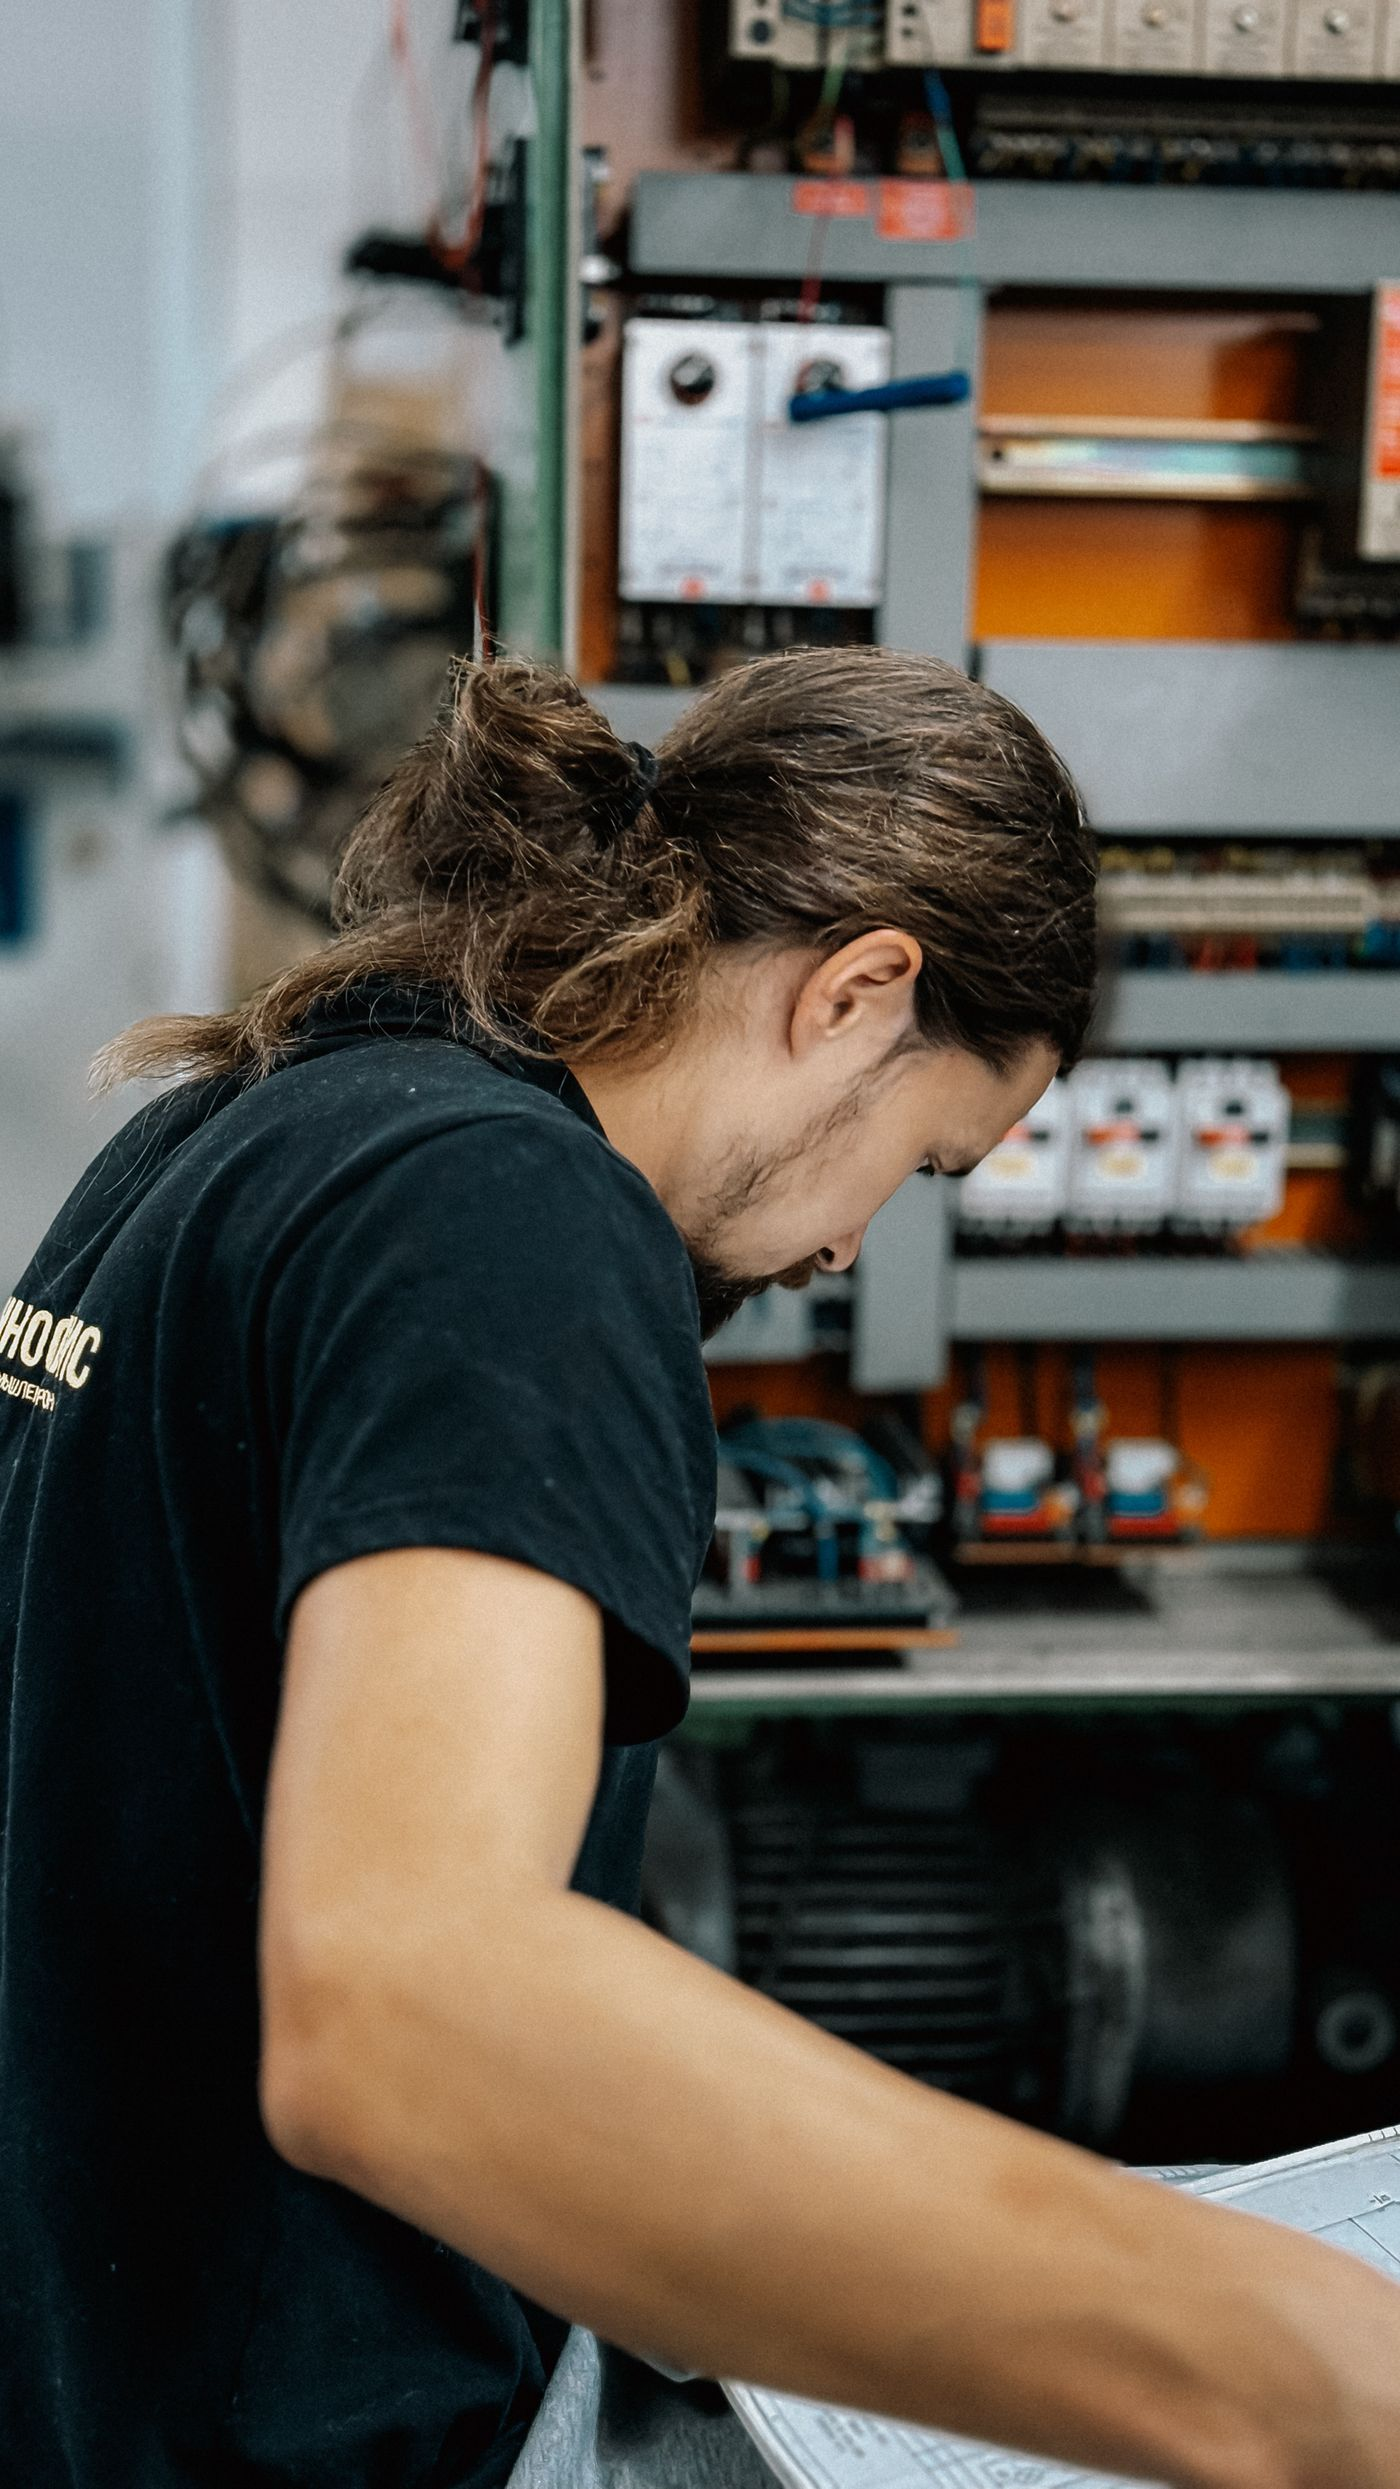
\includegraphics[width=62mm]{../assets/stock/electric-panel.jpg}};
\end{scope}
\labeltext{10}{59}{70}{Оператор и диспетчер}
\bodytext{10}{51}{70}{Принимают заявку, назначают мастера и следят за временем.}
\labeltext{10}{33}{70}{Главный мастер}
\bodytext{10}{25}{70}{Проверяет смету, обучает исполнителей и контролирует сложные случаи.}
\slideend
\end{frame}

\begin{frame}[plain]
\slidebegin{Оплата}{Клиенту не нужно рассчитываться с каждым}{16}
\node[anchor=center,inner sep=0] at (119,40) {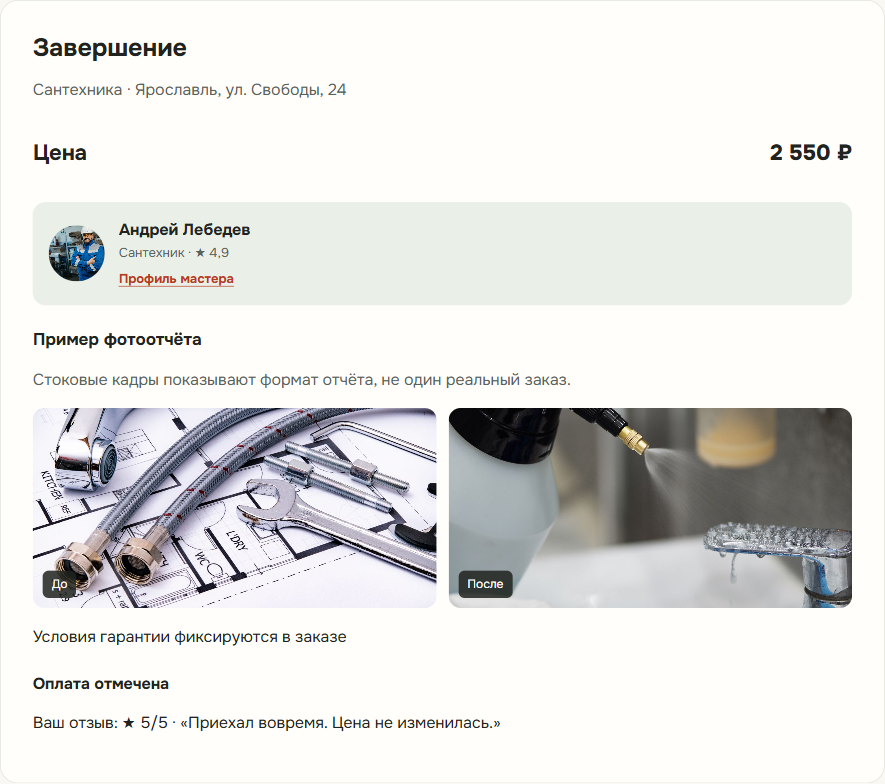
\includegraphics[width=61mm,height=48mm,keepaspectratio]{site-estimate.png}};
\labeltext{10}{59}{70}{Единый заказ}
\bodytext{10}{51}{70}{Сумма и состав работ видны до выезда. После ремонта — одна оплата.}
\labeltext{10}{33}{70}{Сейчас}
\bodytext{10}{25}{70}{В прототипе оплата условная; реальный платёжный сервис ещё подключить.}
\slideend
\end{frame}

\begin{frame}[plain]
\slidebegin{Пилот}{Проверим обещания на реальных заказах}{17}
\labeltext{10}{61}{138}{Скорость}
\bodytext{10}{53}{138}{Время от заявки до ответа и от заявки до приезда по каждому району.}
\labeltext{10}{44}{138}{Цена}
\bodytext{10}{36}{138}{Сколько смет меняется после осмотра и почему.}
\labeltext{10}{27}{138}{Качество}
\bodytext{10}{19}{138}{Повторные обращения, выполнение чек-листа и отзывы клиентов.}
\slideend
\end{frame}

\begin{frame}[plain]
\begin{tikzpicture}[remember picture,overlay,x=1mm,y=1mm]
\begin{scope}[shift={(current page.south west)}]
\fill[Paper] (0,0) rectangle (160,90);
\node[anchor=west,text=Coral,font=\bfseries\fontsize{12}{14}\selectfont] at (10,84) {Следующий шаг};
\node[anchor=north west,text width=73mm,align=left,text=Ink,font=\bfseries\fontsize{23}{27}\selectfont] at (10,64) {Пилот в Ярославле};
\node[anchor=north west,text width=72mm,align=left,text=Ink,font=\fontsize{12}{16}\selectfont] at (10,41) {Набираем дежурных мастеров, подключаем звонки и оплату, запускаем первые заявки. Проверяем скорость, точность сметы и качество ремонта.};
\node[anchor=center,inner sep=0] at (119,44) {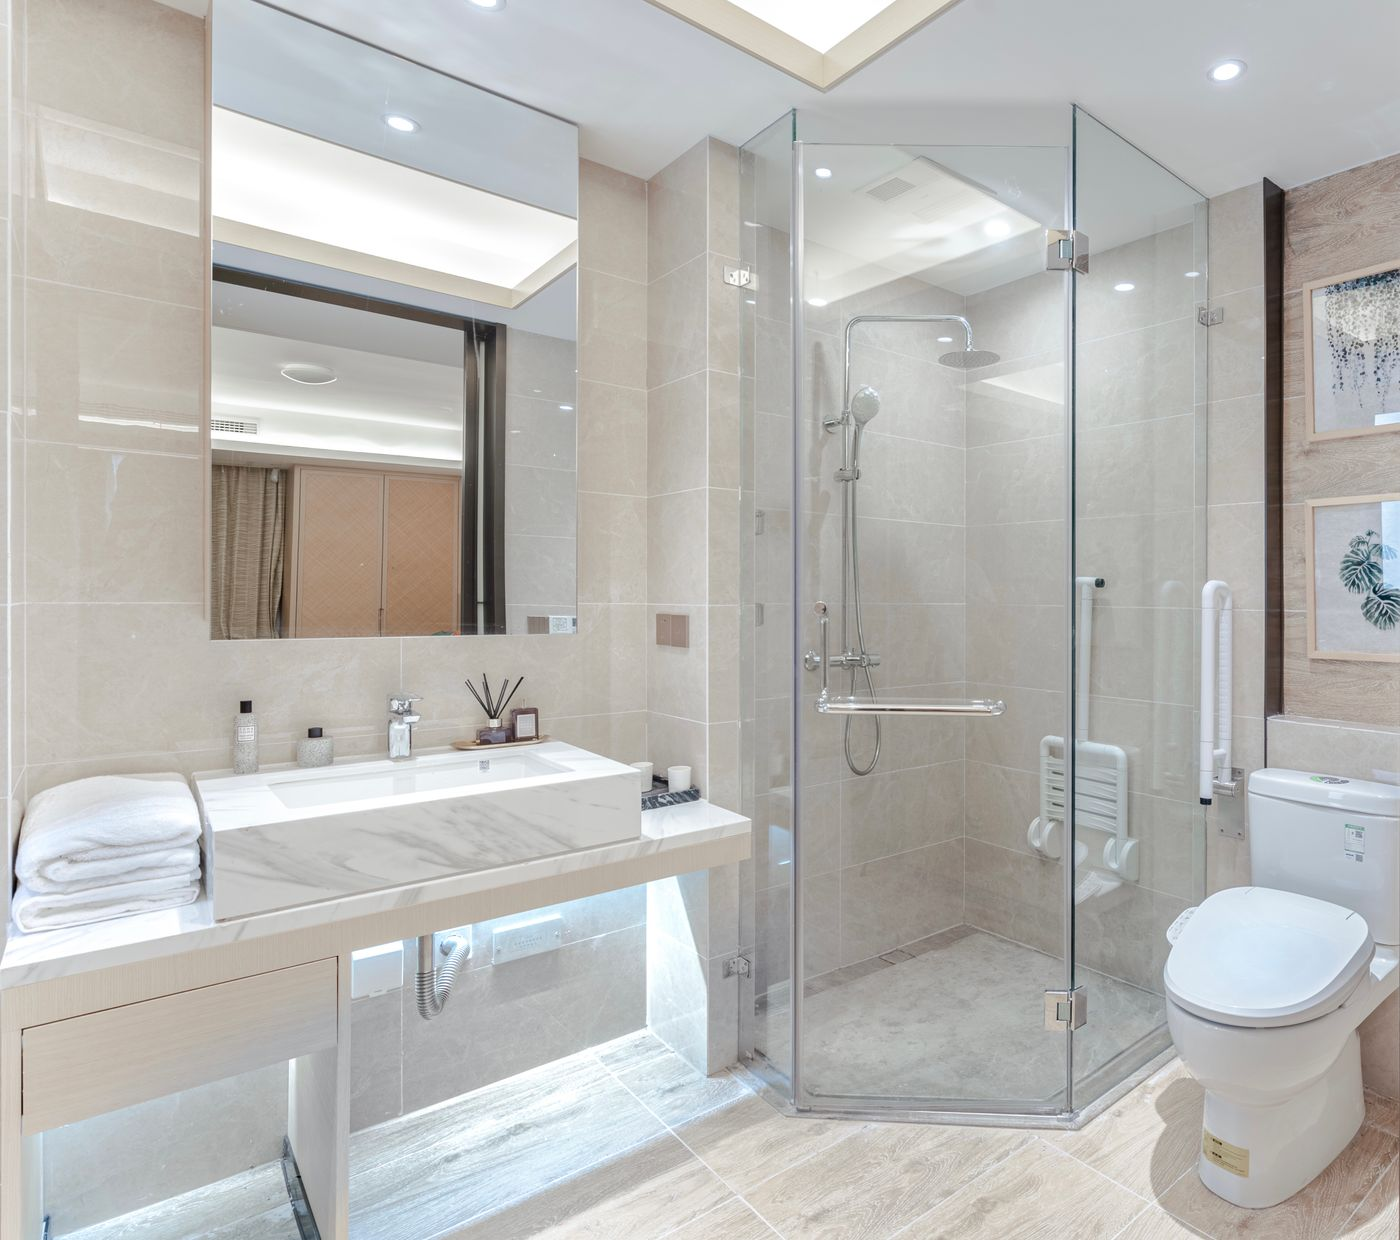
\includegraphics[width=62mm,height=59mm,keepaspectratio]{../assets/stock/bathroom.jpg}};
\end{scope}\end{tikzpicture}\end{frame}

\end{document}
